% ═══════════════════════════════════════════════════════════════════
% EEP: Partner presentation (20 frames: title, problem+w CFO sketch, merged EEP/stack, gates\dots use cases, 3-in-1 patterns, CTA)
% Compile with pdflatex on Overleaf. No special fonts needed.
% ═══════════════════════════════════════════════════════════════════
\documentclass[aspectratio=169,10pt]{beamer}

% ─── Theme ───────────────────────────────────────────────────────
\usetheme{default}
\useinnertheme{rectangles}

% ─── Colors ──────────────────────────────────────────────────────
\definecolor{bg}{HTML}{0B0F1A}
\definecolor{card}{HTML}{141926}
\definecolor{accent}{HTML}{6366F1}
\definecolor{cyan}{HTML}{22D3EE}
\definecolor{mint}{HTML}{34D399}
\definecolor{rose}{HTML}{FB7185}
\definecolor{amber}{HTML}{FBBF24}
\definecolor{slate}{HTML}{94A3B8}
\definecolor{txtw}{HTML}{F1F5F9}
\definecolor{txtm}{HTML}{CBD5E1}
\definecolor{cardbg}{HTML}{1E293B}

\setbeamercolor{normal text}{fg=txtw,bg=bg}
\setbeamercolor{structure}{fg=accent}
\setbeamercolor{frametitle}{fg=txtw,bg=bg}
\setbeamercolor{block title}{fg=txtw,bg=cardbg}
\setbeamercolor{block body}{fg=txtm,bg=card}
\setbeamercolor{itemize item}{fg=accent}
\setbeamercolor{itemize subitem}{fg=cyan}

% ─── Layout ──────────────────────────────────────────────────────
\setbeamertemplate{navigation symbols}{}
\setbeamertemplate{footline}{%
  \hfill\textcolor{slate}{\scriptsize\insertframenumber\,/\,\inserttotalframenumber}%
  \hspace{10pt}\vspace{6pt}%
}
\setbeamertemplate{frametitle}{%
  \vspace{10pt}%
  {\usebeamerfont{frametitle}\usebeamercolor[fg]{frametitle}\insertframetitle}%
  \ifx\insertframesubtitle\empty\else\\[1pt]%
    {\usebeamerfont{framesubtitle}\textcolor{slate}{\insertframesubtitle}}%
  \fi%
  \vspace{4pt}%
}
\setbeamerfont{frametitle}{size=\large,series=\bfseries}
\setbeamerfont{framesubtitle}{size=\footnotesize}
\setbeamertemplate{itemize items}[circle]

\setbeamersize{text margin left=20pt, text margin right=20pt}

% ─── Packages ────────────────────────────────────────────────────
\usepackage[utf8]{inputenc}
\usepackage[T1]{fontenc}
\usepackage{lmodern}
\usepackage{array}
\usepackage{booktabs}
\usepackage{tikz}
\usetikzlibrary{shapes.geometric,arrows.meta,positioning}
\usepackage{hyperref}
\usepackage{pifont}

\hypersetup{colorlinks=true, linkcolor=cyan, urlcolor=cyan}

% ─── Helpers ─────────────────────────────────────────────────────
\newcommand{\hi}[1]{\textcolor{accent}{\textbf{#1}}}
\newcommand{\cmark}{\textcolor{mint}{\ding{51}}}
\newcommand{\xmark}{\textcolor{rose}{\ding{55}}}
\newcommand{\badge}[2]{\colorbox{#1!15!bg}{\footnotesize\textcolor{#1}{\textbf{#2}}}}

% ═══════════════════════════════════════════════════════════════════
\begin{document}

% ─── SLIDE 1 / 11: Title ─────────────────────────────────────────
{
\setbeamertemplate{footline}{}
\begin{frame}[plain]
\begin{tikzpicture}[remember picture,overlay]
  \fill[bg] (current page.south west) rectangle (current page.north east);
  \fill[accent,opacity=0.06] (current page.center) ++(3,1) circle (7);
  \fill[cyan,opacity=0.04] (current page.south west) ++(3,2) circle (4);
\end{tikzpicture}
\vspace{1cm}
\begin{center}
  {\scriptsize\color{cyan}\texttt{OPEN PROTOCOL\quad\textperiodcentered\quad APACHE 2.0}}\par
  \vspace{0.7cm}
  {\fontsize{30}{36}\selectfont\color{txtw}\textbf{Entity Engagement Protocol}\par}
  \vspace{0.8cm}
  {\normalsize\color{slate}Discovery, push events, and machine-verifiable access, with reference deployments and conformance tooling you can run today.\par}
  \vspace{0.5cm}
  {\normalsize\color{txtm}\textbf{Dr.\ Ugur Cekmez}\par}
  \vspace{0.5cm}
  {\scriptsize\color{slate}\texttt{eep.dev}\qquad March 2026}\par
\end{center}
\end{frame}
}


% ─── SLIDE 2 / 11: The Problem ───────────────────────────────────
\begin{frame}[shrink=5]{The web wasn't built for agents}
\framesubtitle{Agents scrape, poll, and guess. You get burned compute, burned tokens, and no shared rules for machines.}

\vspace{0.15cm}

\begin{columns}[T]
\begin{column}{0.46\textwidth}
{\footnotesize\color{rose} TODAY'S REALITY}\par
\vspace{5pt}
{\small\color{txtm}%
An agent visiting a website downloads kilobytes of HTML, CSS, and JS to find a single data point.\par
\vspace{4pt}
\hi{80\% of every token} is wasted on layout the agent will never see.\par
\vspace{4pt}
One AI query uses up to 10$\times$ the electricity of a standard search.\par
\vspace{4pt}
When data changes, the agent has no way to know. It polls and hopes.%
}
\end{column}

\begin{column}{0.46\textwidth}
{\footnotesize\color{mint} WHAT AGENTS ACTUALLY NEED}\par
\vspace{5pt}
{\small\color{txtm}%
\cmark\; Structured data, not rendered HTML\par
\vspace{3pt}
\cmark\; Push notifications on changes\par
\vspace{3pt}
\cmark\; Cryptographic identity (W3C \textbf{DIDs}): {\color{slate}\footnotesize a machine passport you cannot fake; not a shared password}\par
\vspace{3pt}
\cmark\; Machine-readable access control\par
\vspace{3pt}
\cmark\; Autonomous commerce\par
\vspace{3pt}
\cmark\; One protocol instead of N integrations\par
}
\vspace{6pt}
{\footnotesize\color{amber}\textbf{Agentic AI market}}\par
\vspace{2pt}
\badge{amber}{\$7.3B (2025) \;$\to$\; \$9.1B (2026) \;$\to$\; \$139B (2034)}\par
\vspace{2pt}
{\scriptsize\color{slate} Source: Fortune Business Insights}
\end{column}
\end{columns}

\vspace{0.2cm}
{\footnotesize\color{amber}\textbf{CFO sketch (illustrative):}\; \textbf{50k} clients poll \texttt{/status} every \textbf{60s} $\Rightarrow$ $\sim$\textbf{833 req/min} of ``nothing changed.'' If the underlying truth updates \textbf{120$\times$/hr}, SSE can push about \textbf{2 events/min} to subscribers for the same facts and far less repeat work. Plug in your own traffic; \texttt{compliance-cli} in staging helps sanity-check the story.}
\end{frame}


% ─── EEP overview = manifest + standards + triple stack (merged) ─
\begin{frame}[shrink=8]{EEP: discovery, the triple stack, and standards}
\framesubtitle{Real-time, verifiable events: Layer~1 state, Layer~2 push, Layer~3 negotiation.}

\vspace{0.06cm}
\begin{center}
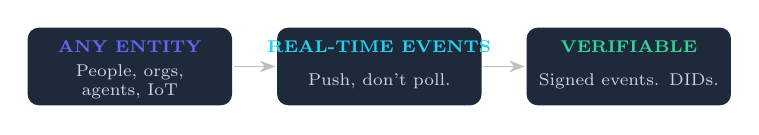
\begin{tikzpicture}[scale=0.88, transform shape,
  card/.style={rectangle, rounded corners=4pt, minimum width=2.95cm,
               minimum height=1.12cm, fill=cardbg, align=center},
  clbl/.style={font=\scriptsize\bfseries},
  cdsc/.style={font=\scriptsize, text=txtm, text width=2.62cm, align=center},
]
\node[card] (c1) at (0,0) {};
\node[clbl, text=accent] at (0,0.28) {ANY ENTITY};
\node[cdsc] at (0,-0.22) {People, orgs, agents, IoT};

\node[card] (c2) at (3.6,0) {};
\node[clbl, text=cyan] at (3.6,0.28) {REAL-TIME EVENTS};
\node[cdsc] at (3.6,-0.22) {Push, don't poll.};

\node[card] (c3) at (7.2,0) {};
\node[clbl, text=mint] at (7.2,0.28) {VERIFIABLE};
\node[cdsc] at (7.2,-0.22) {Signed events. DIDs.};

\draw[-{Stealth[length=2mm]}, gray!50] (1.5,0)--(2.1,0);
\draw[-{Stealth[length=2mm]}, gray!50] (5.1,0)--(5.7,0);
\end{tikzpicture}
\end{center}

\vspace{0.06cm}
\begin{center}
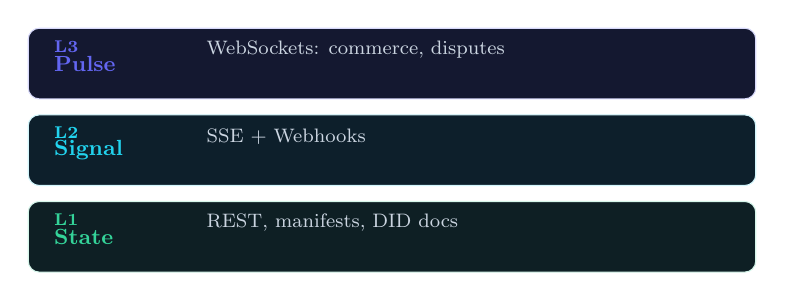
\begin{tikzpicture}[scale=0.88, transform shape,
  layer/.style={rectangle, rounded corners=4pt, minimum width=10.5cm, minimum height=1.02cm},
]
\node[layer, fill=mint!8!bg, draw=mint!20] at (0,0) {};
\node[font={\scriptsize\bfseries}, text=mint, anchor=west] at (-5.0,0.25) {L1};
\node[font={\small\bfseries}, text=mint, anchor=west] at (-5.0,0.0) {State};
\node[font=\footnotesize, text=txtm, anchor=west] at (-2.8,0.2) {REST, manifests, DID docs};
\node[layer, fill=cyan!8!bg, draw=cyan!20] at (0,1.25) {};
\node[font={\scriptsize\bfseries}, text=cyan, anchor=west] at (-5.0,1.5) {L2};
\node[font={\small\bfseries}, text=cyan, anchor=west] at (-5.0,1.25) {Signal};
\node[font=\footnotesize, text=txtm, anchor=west] at (-2.8,1.45) {SSE + Webhooks};
\node[layer, fill=accent!10!bg, draw=accent!25] at (0,2.5) {};
\node[font={\scriptsize\bfseries}, text=accent, anchor=west] at (-5.0,2.75) {L3};
\node[font={\small\bfseries}, text=accent, anchor=west] at (-5.0,2.5) {Pulse};
\node[font=\footnotesize, text=txtm, anchor=west] at (-2.8,2.7) {WebSockets: commerce, disputes};
\end{tikzpicture}
\end{center}

\vspace{0.04cm}
\begin{columns}[T]
\begin{column}{0.48\textwidth}
{\scriptsize\color{accent} DISCOVERY}\par
{\scriptsize\color{txtm}%
\texttt{/.well-known/eep.json}; \texttt{eep.dev} + federated \texttt{eep-registry.json} (economics optional).%
}
\vspace{3pt}
{\tiny\color{slate}%
\textbf{GEO} (industry term for generative-engine optimization): a machine-readable manifest supports structured retrieval for agents and answer engines; it complements classic SEO sitemaps and is not a ranking or placement guarantee.%
}
\end{column}
\begin{column}{0.48\textwidth}
{\scriptsize\color{slate} STANDARDS}\par
{\scriptsize\color{txtm}%
CloudEvents; W3C DIDs / VCs (portable ID + signed claims); RFC~8615; Apache~2.0. Sessions: tokens, delegation, version negotiation.%
}
\end{column}
\end{columns}
\end{frame}


% ─── SLIDE 5 / 11: Gates ─────────────────────────────────────────
\begin{frame}[shrink=3]{Access control that agents understand}
\framesubtitle{Core gate types. \texttt{Combined} stacks several requirements into one atomic verify. No human in the loop.}

\vspace{0.1cm}

\begin{center}
\renewcommand{\arraystretch}{1.25}
{\footnotesize
\begin{tabular}{c l l l}
\toprule
& \textcolor{txtw}{\textbf{Gate}} & \textcolor{slate}{\textbf{Agent provides}} & \textcolor{slate}{\textbf{Use case}} \\
\midrule
\textcolor{mint}{$\circ$} & Public & Nothing & Open knowledge base \\
\textcolor{accent}{$\bullet$} & Identity & DID ownership proof & Know-your-peer \\
\textcolor{cyan}{$\star$} & Credential & W3C Verifiable Credential & Verified researchers only \\
\textcolor{amber}{$\dagger$} & Agreement & Signed license hash & Non-commercial license \\
\textcolor{accent}{$\leftrightarrow$} & Data exchange & Verifiable Presentation & Reciprocal data sharing \\
\textcolor{rose}{\$} & Payment & On-chain tx hash & Per-query micropayment \\
\textcolor{accent}{$\oplus$} & Combined & Satisfy nested reqs (AND/OR) & Pay + sign terms together \\
\bottomrule
\end{tabular}
}
\end{center}

\vspace{0.2cm}

\begin{columns}[T]
\begin{column}{0.46\textwidth}
{\footnotesize\color{txtm}%
Agents that lack the right credential get a structured \texttt{402} response explaining exactly what's missing and how to obtain it.\par
\vspace{3pt}
No forms. No emails. Fully automated.%
}
\end{column}
\begin{column}{0.46\textwidth}
{\footnotesize\color{slate} PARTNER QUESTION}\par
\vspace{2pt}
{\footnotesize\color{txtm}%
\textit{``Can I monetize my API for agents?''}\par
\vspace{2pt}
Yes. \textbf{Payment gate} = verifiable settlement proof (often on-chain tx hash; e.g.\ \textbf{x402}). \textbf{Per-query} micropayments without card rails or MoR billing for autonomous clients.\par
\vspace{3pt}
You set price + chain; agent retries with proof. \textbf{Cryptographic receipt} for revenue + audit.%
}
\end{column}
\end{columns}
\end{frame}


% ─── SLIDE 6 / 11: Commerce ──────────────────────────────────────
\begin{frame}{Agents that negotiate, pay, and settle}
\framesubtitle{Commerce over Layer~3 follows a small state machine. After \textbf{paid}, \texttt{commerce.dispute.*} uses signed artifacts and timestamps (evidence, not an email thread). Three pricing modes. Non-custodial wallets.}

\vspace{0.2cm}

\begin{center}

\begin{tikzpicture}[
  st/.style={rectangle, rounded corners=4pt, minimum width=1.75cm, minimum height=0.72cm,
             fill=cardbg, draw=accent!25, font=\footnotesize\bfseries, text=txtw},
  ar/.style={-{Stealth[scale=0.7]}, thick, color=accent!40},
]
\node[st] (o) at (0,0) {Offer};
\node[st] (c) at (2.6,0) {Counter};
\node[st] (a) at (5.2,0) {Accept};
\node[st] (i) at (7.8,0) {Invoice};
\node[st, draw=mint!30] (p) at (10.4,0) {\textcolor{mint}{Paid}};
\draw[ar] (o)--(c); \draw[ar] (c)--(a); \draw[ar] (a)--(i); \draw[ar] (i)--(p);
\draw[ar, dashed, bend right=25, color=slate!30] (c) to (o);
\end{tikzpicture}
\end{center}

\vspace{2pt}
{\centering\scriptsize\color{slate} After \textbf{Paid}: Layer~3 supports structured disputes (refund, resume, penalty) via \texttt{commerce.dispute.*} envelopes.\par}

\vspace{0.12cm}

\begin{columns}[T]
\begin{column}{0.46\textwidth}
{\footnotesize\color{cyan} PRICING MODES}\par
\vspace{3pt}
{\footnotesize\color{txtm}%
\textcolor{cyan}{$\blacktriangleright$}\; \textbf{Fixed:} posted price, take it or leave it\par
\vspace{2pt}
\textcolor{accent}{$\blacktriangleright$}\; \textbf{Negotiated:} agents trade counter-offers\par
\vspace{2pt}
\textcolor{amber}{$\blacktriangleright$}\; \textbf{Auction:} competitive bidding\par
\vspace{5pt}
Payment settles on-chain (x402). Both sides get a cryptographic receipt. No intermediary.%
}
\end{column}
\begin{column}{0.46\textwidth}
{\footnotesize\color{accent} AGENT WALLETS}\par
\vspace{3pt}
{\footnotesize\color{txtm}%
Agents hold non-custodial wallets with operator-defined spending limits.\par
\vspace{3pt}
Three key isolation models:\par
\vspace{2pt}
{\scriptsize\textcolor{slate}{1.}}\; Operator-derived keys\par
\vspace{1pt}
{\scriptsize\textcolor{slate}{2.}}\; Hardware-backed (TEE)\par
\vspace{1pt}
{\scriptsize\textcolor{slate}{3.}}\; OS keychain\par
\vspace{3pt}
Sub-agents can only spend within the scope their owner delegated.%
}
\end{column}
\end{columns}
\end{frame}


% ─── Security ────────────────────────────────────────────────────
\begin{frame}[shrink=5]{Zero-trust security, by default}
\framesubtitle{No interaction is implicitly trusted. Every request must present cryptographic proof.}

\vspace{0.08cm}
{\footnotesize\color{slate}\textbf{Biz translation:}\; \textbf{mTLS / TLS 1.3} = encrypted pipes + strong server identity; \textbf{DID signatures} = caller proves control of a key, not just possession of a copied API key.}

\vspace{0.12cm}

\begin{columns}[T]
\begin{column}{0.46\textwidth}
{\footnotesize\color{mint} ENFORCED AT THE PROTOCOL LEVEL}\par
\vspace{4pt}
{\footnotesize\color{txtm}%
\cmark\; TLS 1.3+ on every connection\par
\vspace{2pt}
\cmark\; DID-based identity (EdDSA / ES256K)\par
\vspace{2pt}
\cmark\; HMAC-SHA256 signed webhooks\par
\vspace{2pt}
\cmark\; Single-use nonces, 60-second window\par
\vspace{2pt}
\cmark\; Rate limiting per DID, not per IP\par
\vspace{2pt}
\cmark\; Progressive trust: new DIDs start in stricter buckets; \textbf{cold-start} $\to$ \textbf{standard} via VC, conformance, or micropayment (policy-defined)\par
\vspace{2pt}
\cmark\; Constant-time verification\par
\vspace{2pt}
\cmark\; On-chain double-spend prevention%
}
\end{column}

\begin{column}{0.46\textwidth}
{\footnotesize\color{accent} PRIVACY BY DESIGN}\par
\vspace{4pt}
{\footnotesize\color{txtm}%
\cmark\; Data requests declare purpose (W3C DPV)\par
\vspace{2pt}
\cmark\; Publishers set retention limits per claim\par
\vspace{2pt}
\cmark\; Agents withdraw data programmatically\par
\vspace{2pt}
\cmark\; Operators set standing privacy rules\par
\vspace{2pt}
\cmark\; Delegation chains inherit privacy: sub-agents bind to \texttt{operator\_privacy\_policy\_hash} and purpose caps\par
}
\vspace{6pt}
{\footnotesize\color{cyan} POST-QUANTUM READY}\par
\vspace{2pt}
{\footnotesize\color{txtm}%
Hybrid signatures: classical EdDSA plus quantum-safe ML-DSA (NIST FIPS 204). Run both now; keep both on the roadmap for when cryptographically relevant quantum machines show up.%
}
\end{column}
\end{columns}
\end{frame}


% ─── Compliance ───────────────────────────────────────────────────
\begin{frame}[shrink=5]{Regulatory compliance is structural, not bolted on}
\framesubtitle{\textbf{Regulatory shield:} evidence an auditor can replay, not a slide deck full of promises. GDPR, EU AI Act, DORA, eIDAS 2.0.}

\vspace{0.04cm}
{\scriptsize\color{txtm}%
\textbf{Agreement gate:} signed license hash (DID), not browse-wrap. \textbf{Disputes:} \texttt{commerce.dispute.*} + evidence URIs/hashes.%
}

\vspace{0.12cm}

\begin{center}
\renewcommand{\arraystretch}{1.3}
{\footnotesize
\begin{tabular}{l l}
\toprule
\textcolor{txtw}{\textbf{Regulation}} & \textcolor{slate}{\textbf{What EEP provides}} \\
\midrule
\textbf{GDPR / CCPA} & Purpose declarations, retention limits, programmatic data withdrawal \\
\textbf{EU AI Act} & Delegation proofs, full audit trails, human oversight via Operator Policies \\
\textbf{DORA} & mTLS, DID authentication, signed payloads, session revocation \\
\textbf{eIDAS 2.0} & Native W3C VC support, aligned with EU digital identity wallets \\
\bottomrule
\end{tabular}
}
\end{center}

\vspace{0.28cm}

\begin{columns}[T]
\begin{column}{0.46\textwidth}
{\footnotesize\color{accent} CONFORMANCE TIERS}\par
\vspace{3pt}
{\footnotesize\color{txtm}%
\textbf{Core:} Layer 2 events + DID identity\par
\vspace{2pt}
\textbf{Standard:} Core + Layer 1 + gates\par
\vspace{2pt}
\textbf{Full:} Standard + Layer 3 + commerce\par
\vspace{4pt}
Run \texttt{@eep-dev/compliance-cli} for probes + JSON/Markdown audit reports; optional checks for registry economics, trust status, and delegation binding on reference-grade stacks.%
}
\end{column}
\begin{column}{0.46\textwidth}
{\footnotesize\color{cyan} GOVERNANCE \& FEDERATION}\par
\vspace{3pt}
{\footnotesize\color{txtm}%
EEP evolves through the EEIP process (EEP Improvement Proposals). Public, transparent, community-driven.\par
\vspace{3pt}
\textbf{Be your own registry:} publish \texttt{eep-registry.json}; set trust scope, Sybil rules, optional \textbf{economics}; federation credentials keep it interoperable.%
}
\end{column}
\end{columns}
\end{frame}


% ─── Interoperability ─────────────────────────────────────────────
\begin{frame}{Works with what you already have}
\framesubtitle{No rip-and-replace: EEP is \textbf{additive}. Keep Kong / Apigee / AWS API Gateway; add thin middleware + manifests.}

\vspace{0.12cm}

\begin{columns}[T]
\begin{column}{0.46\textwidth}
{\footnotesize\color{accent} ALONGSIDE OTHER PROTOCOLS}\par
\vspace{4pt}
{\footnotesize\color{txtm}%
\textbf{MCP}: Shipped \textbf{EEP--MCP bridges} (Node/Python): keep your MCP tools; add EEP identity, discovery, and gates without rewriting core backends.\par
\vspace{4pt}
\textbf{OpenAPI}: Your endpoints keep their OpenAPI specs. EEP adds how agents discover and authenticate.\par
\vspace{4pt}
\textbf{ActivityPub / AT Protocol}: Social platforms can expose EEP endpoints alongside existing feeds.%
}
\end{column}

\begin{column}{0.46\textwidth}
{\footnotesize\color{cyan} EXISTING API GATEWAYS}\par
\vspace{4pt}
{\footnotesize\color{txtm}%
Kong, Apigee, AWS API Gateway: deploy thin \textbf{@eep-dev/middleware} (Node) or \textbf{eep-middleware-python}, and add \textbf{@eep-dev/setup-cli} (\texttt{eep-setup}). Use \textbf{init} / \textbf{inject} / \textbf{apply} to scaffold manifests, wrap responses, and map gate proofs:\par
\vspace{3pt}
\cmark\; Adds \texttt{/.well-known/eep.json}\par
\vspace{2pt}
\cmark\; Wraps REST responses with EEP headers\par
\vspace{2pt}
\cmark\; Adds SSE subscription links\par
\vspace{2pt}
\cmark\; Maps gate proofs to existing API keys\par
\vspace{5pt}
{\color{slate}See repo \textbf{five-minute proof} + Compose reference stack: hours-to-days to first verifiable endpoint, not multi-quarter custom programs.}%
}
\end{column}
\end{columns}
\end{frame}


% ─── SLIDE 10 / 11: What Partners Gain ───────────────────────────
\begin{frame}[shrink=8]{What this means for you}
\framesubtitle{Concrete outcomes + \textbf{illustrative} economics to re-model (not a forecast).}

\vspace{0.06cm}

\begin{columns}[T]
\begin{column}{0.46\textwidth}
{\footnotesize\color{mint} NEAR-TERM}\par
\vspace{4pt}
{\footnotesize\color{txtm}%
\textbf{New revenue from agents}\par
{\color{slate} Payment gates + per-query proofs (e.g.\ on-chain hash). \textit{Illustrative:} metered agent access can sit next to human subscriptions; model ARR with your own price sheet.}\par
\vspace{6pt}
\textbf{Cut integration costs}\par
{\color{slate} One manifest surface vs.\ many bespoke connectors. \textit{Illustrative:} deep one-off integrations often run \textbf{\$80k--\$250k} and \textbf{2--4\,qtrs}; setup-cli + middleware aim at \textbf{first manifest + probes in days}, then harden with your metrics.}\par
\vspace{8pt}
\textbf{Real-time data delivery}\par
{\color{slate} Push events to subscribers instead of serving millions of polling requests.}\par
\vspace{10pt}
\textbf{Regulatory readiness}\par
{\color{slate} Built-in compliance with GDPR, EU AI Act, DORA. No separate audit trail layer needed.}%
}
\end{column}

\begin{column}{0.46\textwidth}
{\footnotesize\color{accent} LONGER-TERM}\par
\vspace{4pt}
{\footnotesize\color{txtm}%
\textbf{Agent-to-agent marketplaces}\par
{\color{slate} Specialist agents publish services. Manager agents discover, negotiate, and pay.}\par
\vspace{10pt}
\textbf{Autonomous supply chains}\par
{\color{slate} Subscribe to inventory events. Agents auto-purchase when stock drops below thresholds.}\par
\vspace{10pt}
\textbf{Verifiable reputation}\par
{\color{slate} Cryptographic trust signals replace fakeable reviews and star ratings.}\par
\vspace{10pt}
\textbf{Network effect}\par
{\color{slate} Every entity that adopts EEP makes every other entity more reachable. Early movers shape the standard.}%
}
\end{column}
\end{columns}
\end{frame}


% ═══════════════════════════════════════════════════════════════════
% USE CASES: plain-English partner tone (gist line, then TODAY / WITH EEP).
% ═══════════════════════════════════════════════════════════════════


% ─── How to read the use cases ───────────────────────────────────
\begin{frame}{Use cases: one pattern, seven jobs}
\framesubtitle{Same simple shape on every slide, aimed at product, engineering, and partnership leads.}

\vspace{0.1cm}
{\small\color{txtm}%
Three mechanisms show up again and again:\par
\vspace{4pt}
\textcolor{cyan}{1.}\;\textbf{Push instead of poll:} send an update when state changes so subscribers stop paying for empty ``anything new?'' traffic.\par
\vspace{3pt}
\textcolor{cyan}{2.}\;\textbf{Machine identity} (\textbf{DID}): know \emph{which} agent or integration is calling, not only that \emph{someone} has a secret.\par
\vspace{3pt}
\textcolor{cyan}{3.}\;\textbf{Gates:} identity, payment, agreement, credentials. Policy becomes checks a machine can pass with proofs before data or money moves.\par
}
\vspace{6pt}
{\footnotesize\color{slate} Each slide: \textbf{In plain terms} (one-line gist) $\rightarrow$ \textbf{TODAY} $\rightarrow$ \textbf{WITH EEP}. Same structure, different vertical.}
\end{frame}


% ─── USE CASE 1: Financial Data (A + B) ──────────────────────────
\begin{frame}{Financial data: you're paying for traffic that wastes your servers}
\framesubtitle{Bots ask ``did the price move?'' millions of times; most of the time the answer is ``not yet.''}

\vspace{0.06cm}
{\small\color{amber}\textbf{In plain terms:}\; Most API calls are ``no change yet.'' You still pay to answer every one. \textbf{Push} the tick when the number actually moves; subscribers stop hammering you on a timer.}

\vspace{0.1cm}
\begin{columns}[T]
\begin{column}{0.48\textwidth}
{\small\color{rose} TODAY: what actually happens}\par
\vspace{2pt}
{\small\color{txtm}%
\textbf{1.}\; Bots call your API again and again.\par
\textbf{2.}\; Your computers answer every time, often with ``no change.''\par
\textbf{3.}\; API keys leak; you can't tell a paying customer from a copycat scraper.\par
\textbf{4.}\; Fancy data sits behind screens built for people, not for machines.\par
}
\end{column}

\begin{column}{0.48\textwidth}
{\small\color{mint} WITH EEP: same job, less waste}\par
\vspace{2pt}
{\small\color{txtm}%
\textbf{1.}\; When the price \textbf{really} changes, you \textbf{push} one event (\textbf{SSE}).\par
\textbf{2.}\; Bots subscribe; they don't hammer you on a timer.\par
\textbf{3.}\; A \textbf{payment gate} can charge per look; an \textbf{agreement gate} makes the bot \textbf{sign} your rules first.\par
\textbf{4.}\; Machines can buy premium data the same way people do, only without a human in the loop.\par
}
\end{column}
\end{columns}

\vspace{4pt}
{\footnotesize\color{slate} EEP: SSE push (§5.2) · payment gate (§8) · agreement gate (§8.1) · session persistence (§6)}
\end{frame}


% ─── USE CASE 2: Supply Chain (A) ────────────────────────────────
\begin{frame}{Supply chain: your servers answer the same question millions of times a day}
\framesubtitle{``Has the package moved?'' ``No.'' Same question, same schedule, again. That is most of your traffic.}

\vspace{0.06cm}
{\small\color{amber}\textbf{In plain terms:}\; Tracking endpoints get polled constantly; most replies are ``no update.'' Push \textbf{one event per real status change}; replay for clients that were offline (\texttt{Last-Event-ID}).}

\vspace{0.08cm}
\begin{columns}[T]
\begin{column}{0.48\textwidth}
{\small\color{rose} TODAY: four steps}\par
\vspace{2pt}
{\small\color{txtm}%
\textbf{1.}\; Warehouse software only updates when something happens, but buyers' bots do not see that clock.\par
\textbf{2.}\; So bots ask ``any news?'' on a timer, and mostly hear ``nothing yet.''\par
\textbf{3.}\; Every new trucking partner uses a different system; you rebuild connectors.\par
\textbf{4.}\; A delay happens \emph{now}; the buyer's screen might lag until the next ``ask.''\par
}
\end{column}

\begin{column}{0.48\textwidth}
{\small\color{mint} WITH EEP: four steps}\par
\vspace{2pt}
{\small\color{txtm}%
\textbf{1.}\; Treat each shipment as an \textbf{entity} with a profile.\par
\textbf{2.}\; When status changes, you \textbf{push} one event (\textbf{SSE}) to subscribers.\par
\textbf{3.}\; If a client was offline, \textbf{\texttt{Last-Event-ID}} replays what they missed.\par
\textbf{4.}\; Partners list themselves in a \textbf{manifest/registry}; new partners are \textbf{discoverable}, not custom-wired each time.\par
}
\end{column}
\end{columns}

\vspace{4pt}
{\footnotesize\color{slate} EEP: SSE push + event replay (§5.2) · registry discovery (§4) · content negotiation (§3)}
\end{frame}


% ─── USE CASE 3: SaaS / API Platforms (B) ────────────────────────
\begin{frame}{SaaS: your API has paying customers it doesn't know about}
\framesubtitle{Agents want your data, and there is still no standard machine-readable \textbf{offer} + \textbf{billing} path, so a lot of traffic is scrape-by-default.}

\vspace{0.08cm}
{\small\color{amber}\textbf{In plain terms:}\; Put \textbf{what} you sell and \textbf{how} to pay in a manifest; enforce \textbf{identity}, \textbf{payment}, and \textbf{purpose} before bytes move. One surface for humans and for agents.}

\vspace{0.08cm}
\begin{columns}[T]
\begin{column}{0.48\textwidth}
{\small\color{rose} TODAY: four steps}\par
\vspace{2pt}
{\small\color{txtm}%
\textbf{1.}\; Good data sits behind logins made for browsers, not autonomous software.\par
\textbf{2.}\; Shared API keys blur \textbf{who} is actually calling.\par
\textbf{3.}\; You see traffic spikes; you don't see \emph{who} or \emph{why}.\par
\textbf{4.}\; Honest bots and scrapers look the same from the outside.\par
}
\end{column}

\begin{column}{0.48\textwidth}
{\small\color{mint} WITH EEP: four steps}\par
\vspace{2pt}
{\small\color{txtm}%
\textbf{1.}\; You publish a \textbf{manifest}; agents \textbf{discover} you in the \textbf{registry}.\par
\textbf{2.}\; An \textbf{identity gate} reads the agent's \textbf{DID}: stable identity, not a copied secret.\par
\textbf{3.}\; A \textbf{payment gate} can charge per call; money and access line up.\par
\textbf{4.}\; A \textbf{data-request gate} asks purpose and org type; answers come back \textbf{signed} for audits.\par
}
\end{column}
\end{columns}

\vspace{4pt}
{\footnotesize\color{slate} EEP: identity gate (§8) · payment gate (§8) · data-request gate (§7, §8) · registry (§4)}
\end{frame}


% ─── USE CASE 4: News / Media (B) ───────────────────────────────
\begin{frame}{News: chatbots read your articles for free, then summarize them}
\framesubtitle{Traffic and attribution leak to assistants; paywalls are built for browsers, not autonomous clients.}

\vspace{0.08cm}
{\small\color{amber}\textbf{In plain terms:}\; Treat each article as a \textbf{licensed asset}: price + terms \textbf{before} ingest; cryptographic agreement where a checkbox cannot substitute; \textbf{push} new pieces to subscribers when you publish.}

\vspace{0.08cm}
\begin{columns}[T]
\begin{column}{0.48\textwidth}
{\small\color{rose} TODAY: four steps}\par
\vspace{2pt}
{\small\color{txtm}%
\textbf{1.}\; AI reads your article and hands users the gist; your site may never get the click.\par
\textbf{2.}\; Paywalls expect a \textbf{human} clicking buttons; bots use caches and side doors.\par
\textbf{3.}\; Breaking news reaches search engines late; summaries spread first.\par
\textbf{4.}\; You lose ad money when nobody ``walks through the door.''\par
}
\end{column}

\begin{column}{0.48\textwidth}
{\small\color{mint} WITH EEP: four steps}\par
\vspace{2pt}
{\small\color{txtm}%
\textbf{1.}\; Each article can carry a \textbf{payment gate} (pay per read or subscribe).\par
\textbf{2.}\; An \textbf{agreement gate} makes the bot \textbf{cryptographically sign} ``I will attribute,'' not tick a box nobody audits.\par
\textbf{3.}\; New stories \textbf{push} to subscribers over \textbf{SSE} when you publish, instead of waiting on crawl and index lag.\par
\textbf{4.}\; Money and rules happen \textbf{before} the bot ingests the text.\par
}
\end{column}
\end{columns}

\vspace{4pt}
{\footnotesize\color{slate} EEP: payment gate (§8) · agreement gate (§8.1) · SSE push (§5.2)}
\end{frame}


% ─── USE CASE 5: Enterprise B2B Data Exchange (B + C) ────────────
\begin{frame}{B2B data exchange: why does onboarding still take six weeks?}
\framesubtitle{Each partner still gets a bespoke legal + technical + credential track, even when the \textbf{data product} is the same.}

\vspace{0.08cm}
{\small\color{amber}\textbf{In plain terms:}\; \textbf{Discover} partners through manifests; \textbf{sign} terms and answer purpose and org questions with proofs a machine can check. Fewer one-off connectors, less trust-me theatre.}

\vspace{0.08cm}
\begin{columns}[T]
\begin{column}{0.48\textwidth}
{\small\color{rose} TODAY: four steps}\par
\vspace{2pt}
{\small\color{txtm}%
\textbf{1.}\; Legal drafts NDAs; engineering builds one-off connectors; ops mints keys.\par
\textbf{2.}\; Each partner is a \textbf{custom project}, not a repeatable plug-in.\par
\textbf{3.}\; After go-live you mostly \emph{assume} they follow terms, with little you can machine-check.\par
\textbf{4.}\; When rules change, you replay the whole slow dance.\par
}
\end{column}

\begin{column}{0.48\textwidth}
{\small\color{mint} WITH EEP: four steps}\par
\vspace{2pt}
{\small\color{txtm}%
\textbf{1.}\; Partners publish a \textbf{manifest}; your side \textbf{discovers} them in the \textbf{registry}.\par
\textbf{2.}\; An \textbf{agreement gate}: their agent signs your terms with a \textbf{DID} key. Auditable, not a PDF buried in a thread.\par
\textbf{3.}\; A \textbf{data-request gate} asks org type and purpose; answers return as \textbf{signed credentials}.\par
\textbf{4.}\; Session flows can complete in \textbf{one structured round-trip} instead of weeks of plumbing.\par
}
\end{column}
\end{columns}

\vspace{4pt}
{\footnotesize\color{slate} EEP: agreement gate (§8.1) · data-request gate (§8.2) · registry (§4) · session persistence (§6)}
\end{frame}


% ─── USE CASE 6: Fintech / Banking (C) ──────────────────────────
\begin{frame}{Fintech: an agent just called your API. Who authorized it?}
\framesubtitle{The door opened because someone had a key, but whose key? And are they allowed to open \emph{that} drawer?}

\vspace{0.08cm}
{\small\color{amber}\textbf{In plain terms:}\; A token proves \textbf{possession}. A \textbf{delegation proof} proves \textbf{who} delegated, \textbf{what} scope, and \textbf{when} it expires. Auditors want that chain, not another shared secret.}

\vspace{0.08cm}
\begin{columns}[T]
\begin{column}{0.48\textwidth}
{\small\color{rose} TODAY: four steps}\par
\vspace{2pt}
{\small\color{txtm}%
\textbf{1.}\; You see an API key or token, not the \textbf{human or org} behind the software.\par
\textbf{2.}\; You can't tell \textbf{scope} (read vs pay) or \textbf{expiry} in a standard way.\par
\textbf{3.}\; Compliance teams glue logs together differently for each partner.\par
\textbf{4.}\; New integrations still mean long legal + key ceremonies.\par
}
\end{column}

\begin{column}{0.48\textwidth}
{\small\color{mint} WITH EEP: four steps}\par
\vspace{2pt}
{\small\color{txtm}%
\textbf{1.}\; The agent shows a \textbf{DID}, a stable machine identity.\par
\textbf{2.}\; It adds a \textbf{delegation proof}: who authorized it, what it may do, \textbf{when it ends}.\par
\textbf{3.}\; Requests can be \textbf{signed at the protocol layer}, so audit trails are not an afterthought.\par
\textbf{4.}\; A \textbf{credential gate} can require ``licensed institution'' (or other policy) before data flows.\par
}
\end{column}
\end{columns}

\vspace{4pt}
{\footnotesize\color{slate} EEP: DID identity (§3) · delegation proofs (§13.6) · credential gate (§8) · DORA/eIDAS (§14)}
\end{frame}


% ─── USE CASE 7: IoT / Connected Devices (A + C) ────────────────
\begin{frame}{IoT: your devices could negotiate. They just have no way to.}
\framesubtitle{Devices report through vendor clouds; cross-vendor coordination (e.g.\ grid vs charger) rarely has a direct, policy-bound channel.}

\vspace{0.08cm}
{\small\color{amber}\textbf{In plain terms:}\; Give assets \textbf{DIDs} and \textbf{DNS}-backed discovery; use \textbf{WebSocket} for live negotiation; cap what a device may promise with \textbf{spending controls}. You still get automation, without sneaking around governance.}

\vspace{0.08cm}
\begin{columns}[T]
\begin{column}{0.48\textwidth}
{\small\color{rose} TODAY: four steps}\par
\vspace{2pt}
{\small\color{txtm}%
\textbf{1.}\; Devices mostly talk to \textbf{vendor clouds}, not peer-to-peer.\par
\textbf{2.}\; Another company's agent reaches your gadget only through \textbf{that} vendor's API.\par
\textbf{3.}\; A charger and the grid can't \textbf{directly} agree on timing and price.\par
\textbf{4.}\; Data stays in \textbf{vendor silos} with weak cross-brand paths.\par
}
\end{column}

\begin{column}{0.48\textwidth}
{\small\color{mint} WITH EEP: four steps}\par
\vspace{2pt}
{\small\color{txtm}%
\textbf{1.}\; Give a device a \textbf{DID} + \textbf{DNS TXT} so others can \textbf{find} it without the brand as gatekeeper.\par
\textbf{2.}\; Use \textbf{WebSocket} (Layer 3) for live back-and-forth (``delay 2h, get X'').\par
\textbf{3.}\; \textbf{Spending controls} cap what the device may promise.\par
\textbf{4.}\; Negotiation stays \textbf{machine-native} and \textbf{bounded} by owner policy.\par
}
\end{column}
\end{columns}

\vspace{4pt}
{\footnotesize\color{slate} EEP: DID identity (§3) · DNS discovery (§4.3) · WebSocket negotiation (§5.3) · spending controls (§10.4)}
\end{frame}


% ─── PROTOCOL PATTERNS (three-in-one) ────────────────────────────
\begin{frame}[shrink=6]{Three protocol patterns partners reuse}
\framesubtitle{Delegation chain · pay-then-bytes · evidence-based disputes. Same three moves, many verticals.}

\vspace{0.08cm}
\begin{columns}[T,onlytextwidth]
\begin{column}{0.31\textwidth}
{\small\color{accent}\textbf{1.\ Delegation}}\par
\vspace{2pt}
{\scriptsize\color{txtm}%
Enterprise names who may act; mandate is \textbf{narrow} (actions, resources, \textbf{expiry}). Counterparty verifies principal$\rightarrow$delegate chain. EEP: \textbf{delegation proofs}.%
}
\vspace{2pt}
{\scriptsize\color{slate} proofs · scope · expiry}
\end{column}
\begin{column}{0.31\textwidth}
{\small\color{mint}\textbf{2.\ Quote $\rightarrow$ settle $\rightarrow$ deliver}}\par
\vspace{2pt}
{\scriptsize\color{txtm}%
Publish machine-readable \textbf{terms + price}; client satisfies \textbf{payment gate}; \textbf{then} payload/stream unlocks. Humans and agents: \textbf{pay}, then \textbf{bytes}.%
}
\vspace{2pt}
{\scriptsize\color{slate} 402-style · pricing · settlement proof}
\end{column}
\begin{column}{0.31\textwidth}
{\small\color{cyan}\textbf{3.\ Disagreement}}\par
\vspace{2pt}
{\scriptsize\color{txtm}%
Conflicting outcomes need \textbf{signed artifacts}, timestamps, and a comparison channel, not two JSON files and a shouting match. \texttt{commerce.dispute.*} plus WS: evidence-first reconciliation.%
}
\vspace{2pt}
{\scriptsize\color{slate} disputes · WS · audit trail}
\end{column}
\end{columns}
\end{frame}


% ─── SLIDE: CTA ──────────────────────────────────────────────────
{
\setbeamertemplate{footline}{}
\begin{frame}[plain]
\begin{tikzpicture}[remember picture,overlay]
  \fill[bg] (current page.south west) rectangle (current page.north east);
  \fill[accent,opacity=0.05] (current page.center) ++(3,0) circle (8);
  \fill[cyan,opacity=0.03] (current page.south west) ++(2,2) circle (4);
\end{tikzpicture}
\vspace{1.45cm}
\begin{center}
  {\fontsize{26}{32}\selectfont\color{txtw}\textbf{Let's build this together.}\par}
  \vspace{0.85cm}
  {\color{slate}\rule{4cm}{0.3pt}}\par
  \vspace{0.8cm}
  {\small\color{txtm}%
  \begin{tabular}{rl}
    \textcolor{cyan}{\texttt{web}} & \texttt{eep.dev} \\[6pt]
    \textcolor{cyan}{\texttt{paper}} & \texttt{eep.dev/whitepaper} \\[6pt]
    \textcolor{cyan}{\texttt{github}} & \texttt{github.com/eep-dev} \\[6pt]
    \textcolor{cyan}{\texttt{email}} & \texttt{hello@eep.dev} \\
  \end{tabular}
  }\par
  \vspace{0.6cm}
  {\footnotesize\color{slate}%
    Open source\quad\textperiodcentered\quad Apache 2.0\quad\textperiodcentered\quad TypeScript + Python SDKs}\par
  \vspace{0.15cm}
  {\scriptsize\color{slate}%
    \texttt{npm}:\; @eep-dev/discovery\quad @eep-dev/gates\quad @eep-dev/signer\quad @eep-dev/validator\par
    \vspace{2pt}
    \texttt{pip}:\; eep-discovery\quad eep-gates\quad eep-signer\quad eep-validator}
\end{center}
\end{frame}
}

\end{document}